%
% This is a borrowed LaTeX template file for lecture notes for CS267,
% Applications of Parallel Computing, UCBerkeley EECS Department.
% Now being used for CMU's 10725 Fall 2012 Optimization course
% taught by Geoff Gordon and Ryan Tibshirani.  When preparing 
% LaTeX notes for this class, please use this template.
%
% To familiarize yourself with this template, the body contains
% some examples of its use.  Look them over.  Then you can
% run LaTeX on this file.  After you have LaTeXed this file then
% you can look over the result either by printing it out with
% dvips or using xdvi. "pdflatex template.tex" should also work.
%

\documentclass[twoside]{article}
\setlength{\parindent}{1.5cm}
\setlength{\oddsidemargin}{0.25 in}
\setlength{\evensidemargin}{-0.25 in}
\setlength{\topmargin}{-0.6 in}
\setlength{\textwidth}{6.5 in}
\setlength{\textheight}{8.5 in}
\setlength{\headsep}{0.75 in}
\setlength{\parindent}{0 in}
\setlength{\parskip}{0.1 in}

%
% ADD PACKAGES here:
%

\usepackage{amsmath,amsfonts,graphicx}
\usepackage{algpseudocode}


%
% The following commands set up the lecnum (lecture number)
% counter and make various numbering schemes work relative
% to the lecture number.
%
\newcounter{lecnum}
\renewcommand{\thepage}{\thelecnum-\arabic{page}}
\renewcommand{\thesection}{\thelecnum.\arabic{section}}
\renewcommand{\theequation}{\thelecnum.\arabic{equation}}
\renewcommand{\thefigure}{\thelecnum.\arabic{figure}}
\renewcommand{\thetable}{\thelecnum.\arabic{table}}

%
% The following macro is used to generate the header.
%
\newcommand{\lecture}[4]{
   \pagestyle{myheadings}
   \thispagestyle{plain}
   \newpage
   \setcounter{lecnum}{#1}
   \setcounter{page}{1}
   \noindent
   \begin{center}
   \framebox{
      \vbox{\vspace{2mm}
    \hbox to 6.28in { {\bf STATS 700: Bayesian Inference and Computation
	\hfill Fall 2017} }
       \vspace{4mm}
       \hbox to 6.28in { {\Large \hfill Lecture #1: #2  \hfill} }
       \vspace{2mm}
       \hbox to 6.28in { {\it Lecturer: #3 \hfill Scribes: #4} }
      \vspace{2mm}}
   }
   \end{center}
   \markboth{Lecture #1: #2}{Lecture #1: #2}

   {\bf Note}: {\it LaTeX template courtesy of UC Berkeley EECS dept.}

   {\bf Disclaimer}: {\it These notes have not been subjected to the
   usual scrutiny reserved for formal publications.  They may be distributed
   outside this class only with the permission of the Instructor.}
   \vspace*{4mm}
}
%
% Convention for citations is authors' initials followed by the year.
% For example, to cite a paper by Leighton and Maggs you would type
% \cite{LM89}, and to cite a paper by Strassen you would type \cite{S69}.
% (To avoid bibliography problems, for now we redefine the \cite command.)
% Also commands that create a suitable format for the reference list.
\renewcommand{\cite}[1]{[#1]}
\def\beginrefs{\begin{list}%
        {[\arabic{equation}]}{\usecounter{equation}
         \setlength{\leftmargin}{2.0truecm}\setlength{\labelsep}{0.4truecm}%
         \setlength{\labelwidth}{1.6truecm}}}
\def\endrefs{\end{list}}
\def\bibentry#1{\item[\hbox{[#1]}]}

%Use this command for a figure; it puts a figure in wherever you want it.
%usage: \fig{NUMBER}{SPACE-IN-INCHES}{CAPTION}
\newcommand{\fig}[3]{
			\vspace{#2}
			\begin{center}
			Figure \thelecnum.#1:~#3
			\end{center}
	}
% Use these for theorems, lemmas, proofs, etc.
\newtheorem{theorem}{Theorem}[lecnum]
\newtheorem{lemma}[theorem]{Lemma}
\newtheorem{proposition}[theorem]{Proposition}
\newtheorem{claim}[theorem]{Claim}
\newtheorem{corollary}[theorem]{Corollary}
\newtheorem{definition}[theorem]{Definition}
\newenvironment{proof}{{\bf Proof:}}{\hfill\rule{2mm}{2mm}}

% **** IF YOU WANT TO DEFINE ADDITIONAL MACROS FOR YOURSELF, PUT THEM HERE:

\newcommand\E{\mathbb{E}}

\begin{document}
%FILL IN THE RIGHT INFO.
%\lecture{**LECTURE-NUMBER**}{**DATE**}{**LECTURER**}{**SCRIBE**}
\lecture{8}{November 1 \& 6: Hamiltonian Monte Carlo Sampling}{Yang Cheng}{Wenshi Chen, Yumeng Ma}
%\footnotetext{These notes are partially based on those of Nigel Mansell.}

% **** YOUR NOTES GO HERE:

% Some general latex examples and examples making use of the
% macros follow.  
%**** IN GENERAL, BE BRIEF. LONG SCRIBE NOTES, NO MATTER HOW WELL WRITTEN,
%**** ARE NEVER READ BY ANYBODY.
This lecture's notes illustrate some uses of
various \LaTeX\ macros.  
Take a look at this and imitate.

\section{Do chains congregate?}
 We need to check whether a chain converge to itself and whether chains generated by the same method congregate. If a chain has different mean for its two subchain, the target distribution may have two or more peaks and the chain goes from one to another. If chains with different initial points don't congregate, there also might be two or more peaks in the target distribution. And our estimation with only one chain is not accurate.

For the left picture in Figure 8.1, we can cut a Markov chain into three pieces. Then compare the mean of the first subchain with the mean of the third subchain. The test is described in R package "coda"'s documentation and "geweke.diag" can run the test for us.

The right picture in Figure \ref{chain} is an not converging case. Besides drawing pictures for different chains, we can calculate within-chain variance and between-chain variance, which is mentioned in "MCMC.html" Yang posted in Canvas. If within-chain variance is significantly greater than between-chain variance, the two chains are congregating. If between-chain variance is larger than within-chain variance, the two chains are not congregating.
\begin{figure}
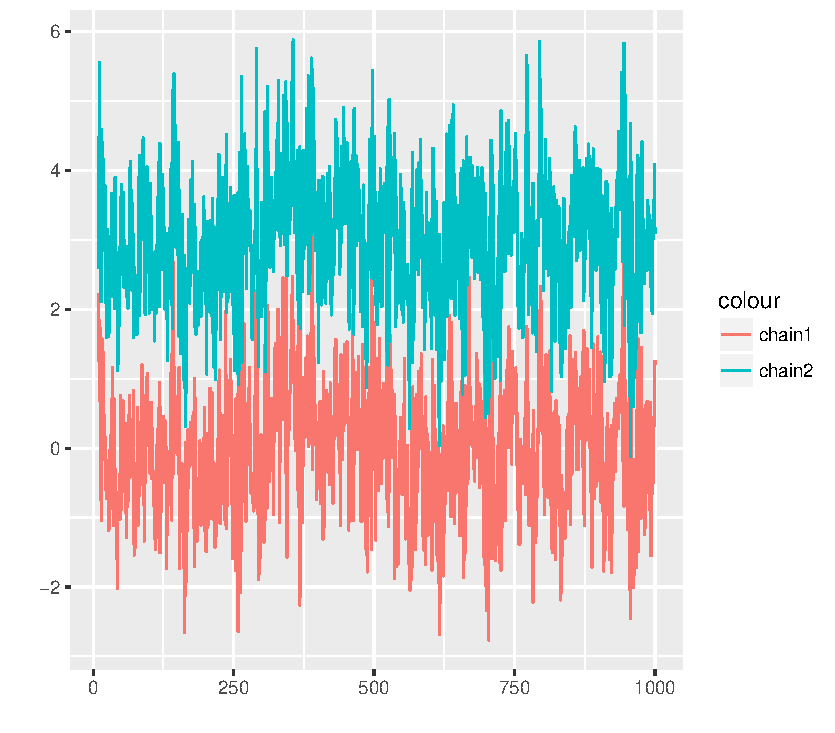
\includegraphics[scale=0.6]{Rplot1.pdf}
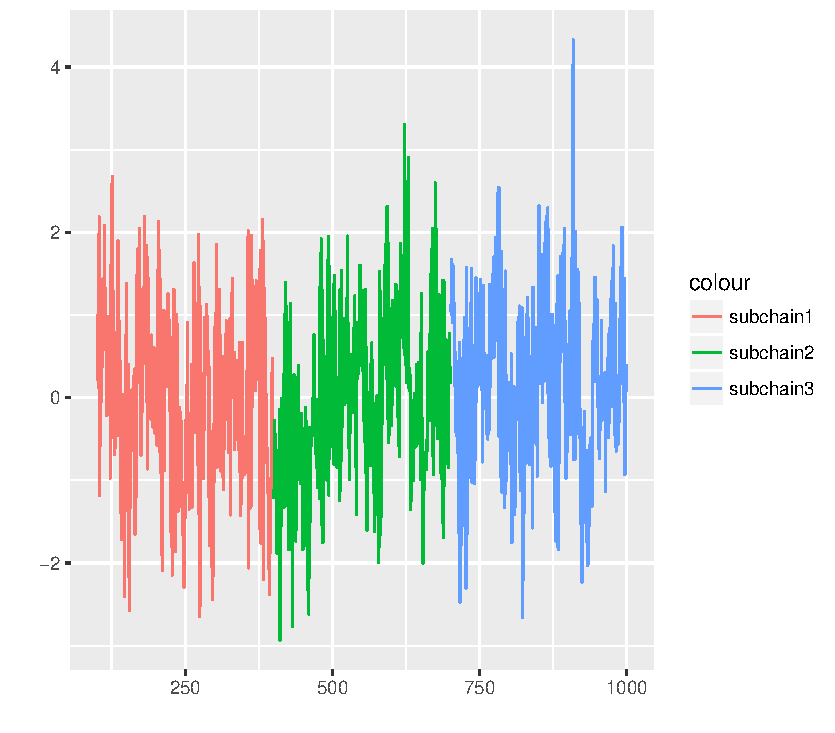
\includegraphics[scale=0.6]{Rplot2.pdf}
\caption{Sampling Path}
\label{chain}
\end{figure}

\section{Hamiltonian Monte Carlo Sampling: Motivation}
Monte Carlo Sampling algorithms covered in previous lectures are related to random walk to various extents. We desire for a more heuristic way to sample the distribution. Ideally, we expect the sampler to move faster at low-probability region and towards high-probability region. Such a sampling system is a close analogy to a Hamiltonian system, with probability density analogous to potential energy and sampler update analogous to momentum. Similarly, we can derive a Monte Carlo sampling algorithm based on Hamiltonian mechanics of a particle.

\section{Hamiltonian Monte Carlo Sampling: Theory}
A Hamiltonian system is described by a function of momentum $p$ and position $q$, known as the Hamiltonian $H(p,q)=K(p)+U(q)$, where $K(p)$ and $U(q)$ represents "kinetic" and "potential" energy respectively. Based on theories in statistical physics, the canonical distribution of state $(p,q)$ has the joint density of 
\begin{equation}
P(p,q)=\frac{1}{Z}\exp\left(\frac{-H(p,q)}{T}\right)=\frac{1}{Z}\exp\left(\frac{-U(q)}{T}\right)\exp\left(\frac{-K(p)}{T}\right).
\end{equation}
Here $Z$ is normalizing constant and $T$ is the "temperature" of the system. We can express the posterior distribution using potential energy function
\begin{equation}
U(q)=-\log\left[\pi(q)L(q|D)\right]
\end{equation}
where $\pi(q)$ is the prior density and $L(q|D)$ is the likelihood given data $D$.

Each step of HMC sampling has two steps. In the first step, new values for the momentum variables are randomly drawn from their Gaussian distribution, independently of the current values of the position variables. For the kinetic energy of Equation 5.23, the d momentum variables are independent, with $p_i$ having zero mean and variance $m_i$. Since $q$ is not changed, and $p$ is drawn from its correct conditional distribution given q (the same as its marginal distribution, due to independence), this step obviously leaves the canonical joint distribution invariant.

\section{Hamiltonian Monte Carlo Sampling: Numerical Scheme}
The evolution of Hamiltonian is governed by Hamiltonian equations
\begin{equation}
\frac{dq_i}{dt}=\frac{\partial H}{\partial p_i}, \frac{dp_i}{dt}=-\frac{\partial H}{\partial q_i}.
\end{equation}
Euler's method is a commonly used numerical scheme for a system of differential equations. Applying Euler's method to the Hamiltonian equations, we obtain:
\begin{eqnarray}
p_i(t+\epsilon)=p_i(t)+\epsilon\frac{dp_i}{dt}=p_i(t)-\epsilon\frac{\partial U}{\partial q_i}(q(t)),\\
q_i(t+\epsilon)=q_i(t)+\epsilon\frac{dq_i}{dt}(t)=q_i(t)+\epsilon\frac{p_i(t)}{m_i}.
\end{eqnarray}
where $\epsilon$ is the time step size. However, Hamiltonian is not conserved under Euler's method. The left plot in Figure \ref{trajectory} shows the trajectory of a Hamiltonian system $H(p,q)=\frac{p^2}{2}+\frac{q^2}{2}$ with initial condition $p=1, q=0$ and time step size $\epsilon=0.3$. Trajectory in the state space of $(p,q)$ simulated from Euler's method diverges quickly from the true trajectory that is a circle. Leapfrog method is preferred in this case for its higher accuracy and conservation of Hamiltonian. The Leapfrog method solves the Hamiltonian equations as follows:
\begin{eqnarray}
p_i(t+\epsilon/2)=p_i(t)-(\epsilon/2)\frac{\partial U}{\partial q_i}(q(t)),\\
q_i(t+\epsilon)=q_i(t)+\epsilon\frac{p_i(t+\epsilon2)}{m_i},\\
p_i(t+\epsilon)=p_i(t+\epsilon/2)-(\epsilon/2)\frac{\partial U}{\partial q_i}(q(t+\epsilon)).
\end{eqnarray}

\begin{figure}
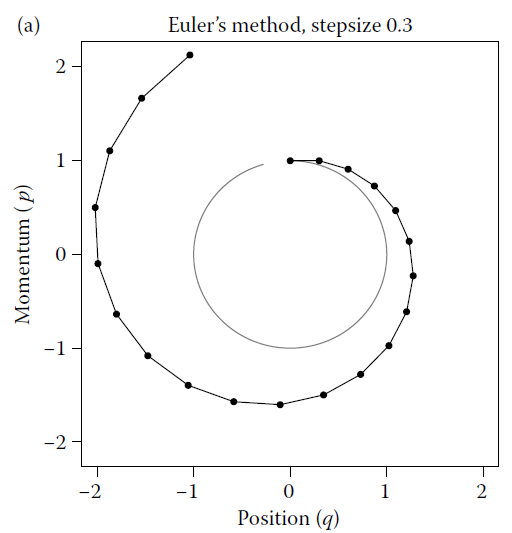
\includegraphics[scale=0.6]{euler.png}
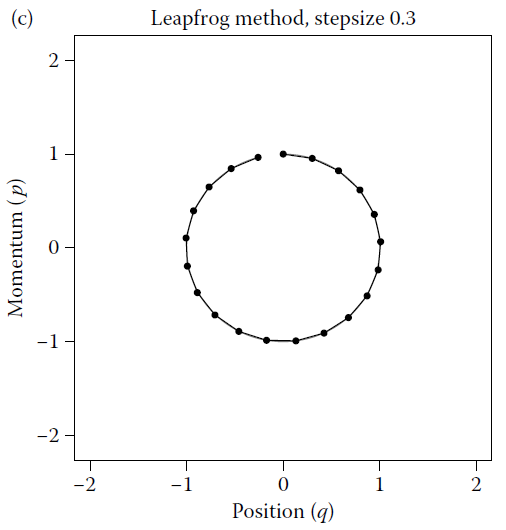
\includegraphics[scale=0.6]{leapfrog.png}
\caption{Trajectory of Hamiltonian Mechanics by Two Methods}
\label{trajectory}
\end{figure}
Combining the Leapfrog method with Hamiltonian analogy, we obtain the Hamiltonian Monte Carlo algorithm updating $(\mathbf{p}^{\text{current}},\mathbf{q}^{\text{current}})$ to $(\mathbf{p}^{\text{next}},\mathbf{q}^{\text{nextt}})$ as follows:
\begin{algorithmic}
\State $n\gets\text{Dimensionality of the Target Distribution}$
\State $L\gets\text{Size of Discretization of the Trajectory}$
\State $\mathbf{q}\gets\mathbf{q}^{\text{current}}$
\For{$i \in \{1,\ldots,n\}$}
\State Sample $p_i$ from $N(0, 1)$
\EndFor
\State $\mathbf{p} \gets \mathbf{p}-\epsilon\frac{\nabla U(\mathbf{q})}{2}$
\State $L\gets\text{Maximum Number of Sampling}$
\For{$i \in \{1,\ldots,L\}$}
\State $\mathbf{q}\gets\mathbf{q}+\epsilon\mathbf{p}$
\If{$i\neq L$}
\State $\mathbf{p}\gets\mathbf{p}-\epsilon\nabla U(\mathbf{q})$
\EndIf
\EndFor
\State $\mathbf{p} \gets \mathbf{p}-\frac{\epsilon}{2}\nabla U(\mathbf{q})$
\State $\mathbf{p}=-\mathbf{p}$
\State $U^{\text{current}}\gets U(\mathbf{q})$
\State $K^{\text{current}}\gets\frac{1}{2}\|\mathbf{p^{\text{current}}}\|^2_2$
\State $U^{\text{proposed}}\gets U(\mathbf{q})$
\State $K^{\text{proposed}}\gets\frac{1}{2}\|\mathbf{p}\|^2_2$
\State Accept $\mathbf{q}$ as $\mathbf{q}^{\text{next}}$ with probability $\min(1,\exp(U^{\text{current}}-U^{\text{proposed}}+K^{\text{current}}-K^{\text{proposed}})$
\end{algorithmic}
The "potential energy" function $U(\mathbf{q})$ is related to the target distribution $p(\mathbf{x}|y)$ by $p(\mathbf{x}|y)=\exp(-U(\mathbf{x}))$. The second loop in the algorithm is essentially performing integral over the contour of $H(\mathbf{p},\mathbf{q})=\text{constant}$.

\section{Hamiltonian Monte Carlo Sampling: Examples}
To demonstrate the power of HMC, we devise a specialized distribution as follows. The observation $(x,y)$ are sampled as $Y\sim N(\theta x,\sigma^2),x\sim N(\theta,1)$. As a result, the log-posterior distribution has
\begin{equation}
\pi_{\sigma}(x,\theta)\propto\exp\left(-\frac{(y-x\theta)^2}{2\sigma^2}-\frac{(x-\theta)^2}{2}\right)\pi_0(\theta),
\end{equation}
where $\pi_0(\theta)$ is the prior distribution. When $\sigma$ is large, the high-probability region is huge and convex. However, when $\sigma$ gets smaller, the shape of high-probability region will resemble crescent moon, which is difficult to sample from with conventional MC algorithms. Figure \ref{sigma} compare the target distribution under different values of $\sigma$.

\begin{figure}
\centering
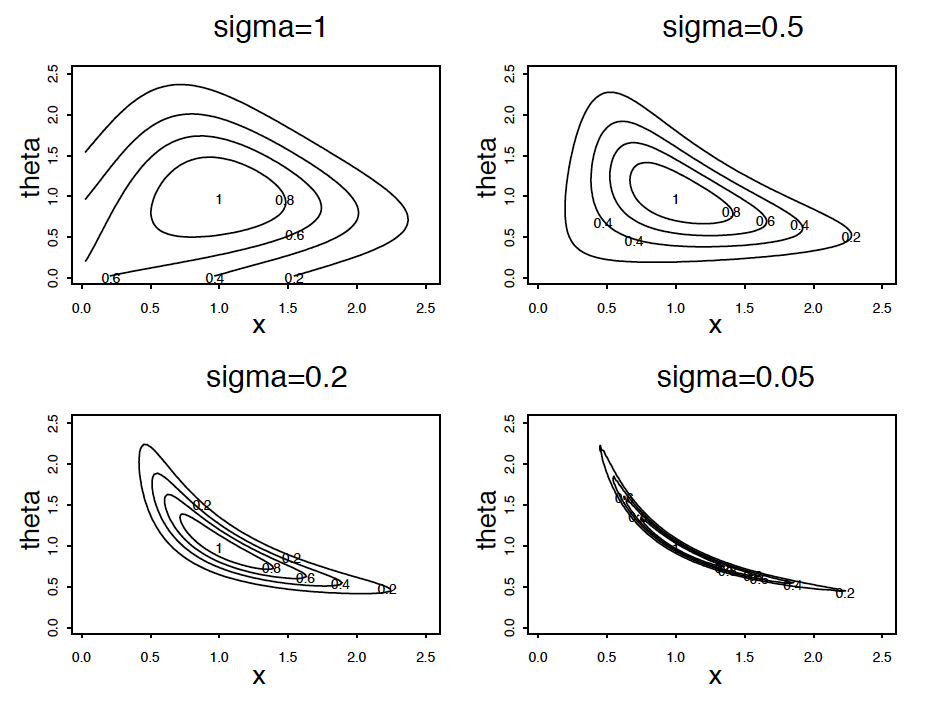
\includegraphics[scale=0.45]{sigma.png}
\caption{Target Distribution under Different $\sigma$}
\label{sigma}
\end{figure}

Now we perform Hamiltonian MC and Metropolis-Hastings MC on this distribution respectively. The maximum number of samples is 5000. Figure \ref{result} shows the results of both methods. The first row shows the result of HMC and the second row shows the MHMC. Comparing the sampling paths of both methods, MHC converges significantly faster than MHMC. After roughly 500 steps, MHC method converges to the target distribution, while in the case of MHMC, the convergence is not reached even after 3000 steps. Hence, this example successfully demonstrate the superior performance of HMC in convergence rate when compared to MHMC.

\begin{figure}
\centering
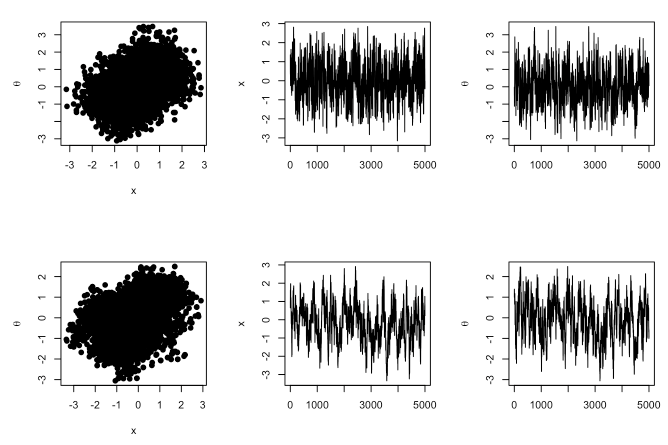
\includegraphics[scale=0.6]{sigma2.png}
\caption{Sampling Results by HMC and MHMC}
\label{result}
\end{figure}

\section*{References}
\beginrefs
\bibentry{1}{\sc R.~Neal}, 
``Chapter 5: MCMC Using Hamiltonian Dynamics,''
{\it Handbook of Markov Chain Monte Carlo}, pp.~113--162.

\bibentry{2}{\sc Yang Chen.}, 
``Special Topics in Applied Statistics,''
{\it Canvas Slides},
University of Michigan, 2017.

\endrefs



% **** THIS ENDS THE EXAMPLES. DON'T DELETE THE FOLLOWING LINE:

\end{document}





